\documentclass[10pt]{article}
\usepackage{icmlko}

\icmlmeta{IP 파운데이션 월드모델}{475}{위약이 아무것도 안 했다}{50노트 만에 문턱을 제대로 재려다, 문턱이 위약으로는 잴 수 없는 물건임을 알았다 --- 그리고 우리 가드 하나가 조용히 헐거워져 있었다}

\begin{document}

\twocolumn[
\icmlheader

\begin{abstract}
이 실험실은 열을 채택할 때 두 가지를 본다. \textbf{위약 6뽑기를
이기는가}, 그리고 \textbf{판 문턱 $0.0045$를 넘는가}. 뒤엣것은
50노트 전에 ``재기선 후 첫 채택 실험에서 짝 부트스트랩으로 다시
재라''고 등록해 두고 미뤄 온 숙제였다. 이번에 이행했더니 답이 아니라
\textbf{질문이 틀렸다}는 것이 나왔다.

위약 여섯을 걸었더니 도메인 $\Delta$가 여섯 다 \textbf{정확히
$0.0000$}이고 뽑기 SD가 $0.00000$이었다. 배선 사고가 아니다 ---
탐욕 분할 부스팅은 \textbf{이득 없는 열을 한 번도 안 가르므로} 나무가
통째로 같아지고 예측이 비트 단위로 일치한다. 연속 잡음
$\cdot$ 이산 잡음 $\cdot$ 마스크 유무 셋 다 확인했다. 결정적 대조:
위약은 진짜 후보와 \emph{값 다중집합이 같고} 배치만 다른데, 진짜는
예측을 바꾸고(spearman $0.744$) 위약은 안 바꾼다. 차이를 만드는 것은
값의 종류가 아니라 \textbf{$y$와의 정렬}이다.

여기서 두 가지가 따라온다. 첫째, \textbf{상수 문턱은 위약으로 잴 수
있는 물건이 아니다} --- 위약 분포가 점질량이라 $2\sigma$가 0이다.
둘째, 더 나쁜 쪽으로, \textbf{위약 가드가 반보수적이 된다}. 위약이
정확히 0이면 \emph{아무 양수나} 6/6을 이긴다. 실제로 아이돌
\texttt{versions}는 위약 6/6을 이기고도 군집 부트 구간이
{$[-0.1790,\,+0.2483]$}로 \textbf{판정 불능}이었다.
\end{abstract}
]

\section{먼저: 그 문턱은 얇은 도메인을 배제한다}

측정 전에 산술부터 했다(직전 사이클이 만든 규약 --- \emph{재기 전에
도달 범위를 계산하라}). 판 $\rho$는 도메인 $\rho$의 \textbf{유보 행수
가중 평균}이므로, 한 도메인에만 붙는 열의 판 $\Delta$는 대략
\emph{그 도메인 가중 $\times$ 도메인 $\Delta$}다. 기지 사례 셋으로
맞춰 봤다: 영화 국적 $0.0577\times0.1075=0.00621$(실제 $+0.0063$),
만화 3열 $0.00158$(실제 $+0.0020$), 모바일 \texttt{n\_device}
$-0.00005$(실제 $0.0000$). 셋 다 맞는다.

그러면 판 문턱 $0.0045$를 넘는 데 필요한 도메인 $\Delta$는
$0.0045/\text{가중}$이다. 웹툰 $0.026$부터 \textbf{아이돌
$0.333$}까지 열두 배 넘게 벌어진다. 최근 채택 아크에서 잰 1열 도메인
효과의 최대가 $0.0577$이니, \textbf{얇은 다섯 도메인의 열은 판
문턱을 구조적으로 못 넘는다.} 그래서 이번 판정은 도메인 수준에서
했고, 판 $\Delta$는 병기만 했다.

\begin{figure}[t]
\centering
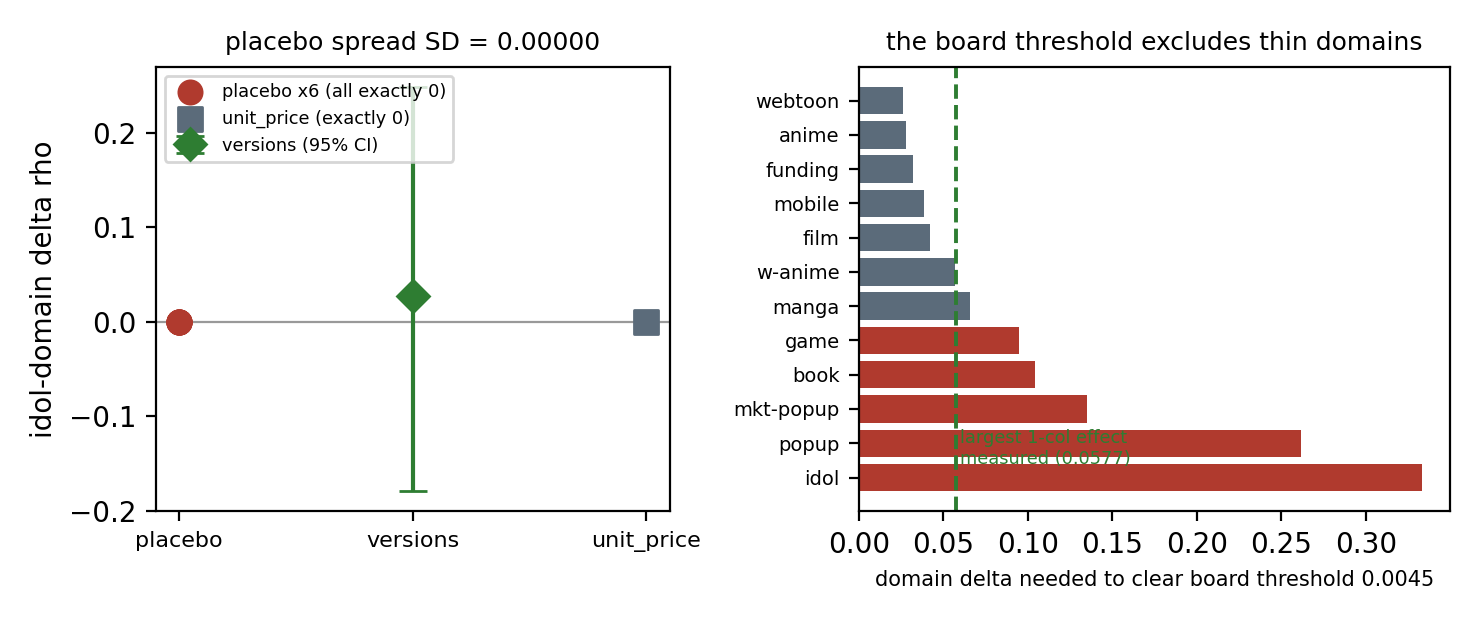
\includegraphics[width=\linewidth]{figs/nullplacebo.png}
\caption{왼쪽: 위약 여섯(빨강)이 한 점에 겹쳐 있다 --- 흩어짐이
아니라 \emph{점}이다. 초록은 유일하게 움직인 후보와 그 95\% 구간.
오른쪽: 판 문턱을 넘는 데 필요한 도메인 $\Delta$. 초록 파선이 이제껏
잰 1열 최대치다. 빨강 막대는 그 선을 넘을 수 없는 도메인들이다.
전부 산출물에서 계산했다.}
\end{figure}

\section{위약이 점질량이면 가드가 헐거워진다}

상시 가드의 문안은 \emph{``위약이 진짜보다 나쁘지 않으면 신호가
아니라 차원 비용이다''}이다. 이 문장은 위약이 \textbf{퍼져 있다}는
것을 조용히 전제한다. 퍼짐이 0이면 문장은 참인 채로 쓸모가 없어진다
--- $+0.0001$도 6/6을 이긴다.

아이돌 \texttt{versions}가 정확히 그 자리에 섰다. 도메인
$\Delta=+0.0278$, 위약 6/6 승. 옛 자로는 통과다. 그런데 프랜차이즈
군집 부트스트랩 구간은 $[-0.1790,\,+0.2483]$ --- 폭이
$0.427$이다(유보 51행 $\cdot$ 41군집). \textbf{두 자가 어긋나고,
헐거운 쪽이 옛 자다.} 규약 47이 모델 짝 비교에서 상수 자를 버린
것과 같은 이유가 한 층 아래 열 채택에도 그대로 있었다.

\texttt{unit\_price}는 더 깨끗하다 --- 도메인 $\Delta$가 정확히
$0$이다. 트리가 그 열을 한 번도 안 갈랐다. 이것은 ``작다''가 아니라
\textbf{``쓰이지 않았다''}이고, 둘은 다른 진술이다.

\section{범위 --- 어디까지 참인가}

이 퇴화는 \textbf{사후 주입 $\cdot$ 단일 도메인} 경로에서 확인된
것이다. 정상 경로는 열이 \emph{공유 인자 공간}에 들어가 다른
도메인까지 흔들고, 실제로 직전 사이클의 영화 값셔플 여섯은
$0.4591$$\sim$$0.4989$로 크게 흩어졌다. 그러니 \emph{``우리 위약은
전부 가짜였다''}로 읽으면 안 된다. 읽어야 할 것은 이것이다:
\textbf{위약을 쓸 때 위약 분포의 폭을 함께 보고, 폭이 0이면 그
가드를 무효로 선언하라.}

내가 이 경로를 쓴 것도 선택이 아니었다. 아이돌은 열두 도메인 중
\textbf{유일하게} 표준 주입이 조용히 중립화된다 --- 아이돌 열
부착부가 달력 $\cdot$ 위키 $\cdot$ 트렌드 제공자만 보고 주입 딕트를
안 읽어서, 이름만 등록되고 값은 통째로 $0.5\cdot$마스크 $0$이 된다.
열두 도메인에 탐침을 넣어 전수로 셌고, 걸린 것은 아이돌 하나다.

\section{교훈}

\textbf{나는 이 사이클의 초판을 통째로 버렸다.} 사전등록에
\emph{``\texttt{\_idol}은 조용히 중립화한다 --- 마스크 합과 값
가짓수를 찍어 확인한다''}라고 적어 놓고, 그 검사를 \textbf{내가 만든
배열}에 걸었다. 마스크 149/173, 값 가짓수 9 --- 전부 참이고 전부
무의미했다. 확인해야 했던 것은 하네스가 \emph{돌려준} 행렬이고,
거기서는 마스크 합이 0이었다. 인용한 노트에 인용하면서 걸렸다.

그래서 규약이 둘 늘었다. \textbf{배선 검사는 입력이 아니라 산출
행렬에 건다}(주입 후 \texttt{A[:,j]}와 \texttt{M[:,j]}를 원본과
대조하는 assert를 러너에 박는다). 그리고 \textbf{위약 6/6을 이겼다는
말만으로 신호를 주장하지 마라} --- 위약의 폭을 함께 보고해라.

이 실험실은 자를 여러 번 고쳐 세웠다. 이번에 배운 것은 조금 다르다:
\emph{자가 틀린 게 아니라, 자가 재던 것이 사라져 있었다.}

\end{document}
